% !TEX root = ../main.tex

\section{Умовні закони розподілу ВВ}

Розглядаємо випадок $n = 2$, $\vec{\xi} = \left(\xi_1, \xi_2\right)^T$.

\begin{definition}
    \emph{Умовним законом розподілу} $\xi_1$ називається закон розподілу 
    $\xi_1$ за умови того, що $\xi_2$ набула відповідного значення (ДВВ) 
    або потрапила в деякий проміжок (НВВ) (для $\xi_2$ аналогічно).
\end{definition}

\begin{definition}
    Універсальним умовним законом розподілу ВВ є \emph{умовна функція 
    розподілу}:
    \begin{equation*}
        F_{\xi_1}(x/y) = P({\xi_1 < x}/{\xi_2 < y}) = 
        \frac{P\left\{\xi_1 < x, \xi_2 < y\right\}}
        {P\left\{\xi_2 < y\right\}} = 
        \frac{F_{\vec{\xi}}(x, y)}{F_{\xi_2}(y)}, F_{\xi_2}(y/x) = \frac{F_{\vec{\xi}}(x, y)}{F_{\xi_1}(x)}
    \end{equation*}
\end{definition}
\begin{remark}
    З означення випливає, що 
    $F_{\vec{\xi}}(x,y) = F_{\xi_1}(x)F_{\xi_2}(y/x)$
    та 
    $F_{\vec{\xi}}(x,y) = F_{\xi_2}(y)F_{\xi_1}(x/y)$.
\end{remark}
\subsection{Умовний закон розподілу дискретного випадкового вектора}
Знову розглядаємо випадок $n=2$ та $\vec{\xi} = (\xi_1, \xi_2)^T$.

Умовні розподіли координат задаються $P\left\{\xi_1 = x_i / \xi_2 = y_j\right\} = 
\frac{P\left\{\xi_1 = x_i , \xi_2 = y_j\right\}}
{P\left\{\xi_2 = y_j\right\}}$ та \\ 
$P\left\{\xi_2 = y_j / \xi_1 = x_i\right\} = 
\frac{P\left\{\xi_1 = x_i , \xi_2 = y_j\right\}}
{P\left\{\xi_1 = x_i\right\}}$.

\begin{example}
    Дискретний випадковий вектор має закон розподілу:

    \begin{tabular}{ccc}
        \begin{tabular}{|c|c|c|c|}
            \hline
            \diagbox{$\xi_2$}{$\xi_1$} & $-1$ & $0$ & $1$\\
            \hline
            0 & $0.1$ & $0.2$ & $0.1$ \\
            \hline
            $1$ & $0.2$ & $0.3$ & $0.1$ \\
            \hline
        \end{tabular}
        &
        \begin{tabular}{|c|c|c|c|}
            \hline
            $\xi_1$ & $-1$ & $0$ & $1$ \\
            \hline
            $p$ & $0.3$ & $0.5$ & $0.2$ \\
            \hline
        \end{tabular}
        &
        \begin{tabular}{|c|c|c|}
            \hline
            $\xi_2$ & $0$ & $1$ \\
            \hline
            $p$ & $0.4$ & $0.5$ \\
            \hline
        \end{tabular}
    \end{tabular}
\end{example}

\begin{tabular}{|c|c|c|c|}
    \hline
    $\xi_1$ & $-1$ & $0$ & $1$ \\
    \hline
    $P\left\{\xi_1 / \xi_2 = 0\right\}$ & $1/4$ 
    & $2/4$ & $1/4$ \\
    \hline
    $P\left\{\xi_1 / \xi_2 = 1\right\}$ & $2/6$ 
    & $3/6$ & $1/6$ \\
    \hline
\end{tabular}
--- умовний закон розподілу $\xi_1$.

\begin{tabular}{|c|c|c|}
    \hline
    $\xi_2$ & $0$ & $1$ \\
    \hline
    $P\left\{\xi_2 / \xi_1 = -1\right\}$ & $1/3$ 
    & $2/3$ \\
    \hline
    $P\left\{\xi_2 / \xi_1 = 0\right\}$ & $2/5$ 
    & $3/5$\\
    \hline
    $P\left\{\xi_2 / \xi_1 = 1\right\}$ & $1/2$ 
    & $1/2$\\
    \hline
\end{tabular}
--- умовний закон розподілу $\xi_2$.

\subsection{Умовне математичне сподівання дискретного випадкового вектора}
\begin{definition}
    \emph{Умовним математичним сподіванням} випадкової величини $\xi_1$ 
    є математичне сподівання цієї випадкової величини за умови, що 
    $\xi_2$ набула певного значення.
    $$E(\xi_1 / \xi_2 = y_j) =
\sum\limits_{i=1}^{n(\infty)}x_i 
P\left\{\xi_1 = x_i / \xi_2 = y_j\right\}, 
E(\xi_2 / \xi_1 = x_i) = \sum\limits_{j=1}^{n(\infty)}y_j 
P\left\{\xi_2 = y_j / \xi_1 = x_i\right\}$$
\end{definition}

\begin{remark}
    Якщо $\xi_1$ та $\xi_2$ незалежні, то $E(\xi_1 / \xi_2 = y_j) 
    = E\xi_1$, $E(\xi_2 / \xi_1 = x_i) = E\xi_2$.
\end{remark}

Умовні математичні сподівання координат дискретного випадкового вектора є дискретними випадковими величинами, оскільки 
приймають декілька значень з певними ймовірностями, тому можна скласти 
їх закон розподілу.
\begin{example}
    Продовження попереднього прикладу:

    \begin{tabular}{c c}
        \begin{tabular}{|c|c|c|}
            \hline
            $E(\xi_1 / \xi_2)$ & $-1/6$ & $0$ \\
            \hline
            $p$ & $0.6$ & $0.4$ \\
            \hline
        \end{tabular}
        &
        \begin{tabular}{|c|c|c|c|}
            \hline
            $E(\xi_2 / \xi_1)$ & $1/3$ & $3/5$ 
            & $1/2$ \\
            \hline
            $p$ & $0.3$ & $0.5$ & $0.2$ \\
            \hline
        \end{tabular}
    \end{tabular}
\end{example}

\begin{equation*}
    D(\xi_1 / \xi_2 = y_j) = 
    E((\xi_1 - E(\xi_1 / \xi_2 = y_j))/\xi_2 = y_j)
\end{equation*}

\subsection{Умовні закони розподілу неперервних випадкових величин}

У випадку $n = 2$, $\vec{\xi} = (\xi_1, \xi_2)^T$: 
\begin{equation*}
    P\{x \leq \xi_1 < x + \Delta x / y \leq \xi_2 < y + \Delta y\} = 
    \frac{P\{\vec{\xi} \in \Pi\}}{P\{y \leq \xi_2 \leq y+\Delta y\}} = 
    \frac{f_{\vec{\xi}}(x,y)\Delta x \Delta y + 
    o(\sqrt{\Delta x^2 + \Delta y^2})}{f_{\xi_2}(y)\Delta y + o(\Delta y)}
\end{equation*}
\begin{definition}
    \emph{Умовною щільністю розподілу} називається функція 
    вигляду:
    \begin{equation*}
        f_{\xi_1}(x/y) = \frac{f_{\vec{\xi}}(x, y)}{f_{\xi_2}(y)}, f_{\xi_2}(y/x) = \frac{f_{\vec{\xi}}(x, y)}{f_{\xi_1}(x)}
    \end{equation*}
\end{definition}

\begin{remark}
    Графік умовно щільність розподілу можна інтерпретувати лінію перетину 
    поверхні розподілу та площини $y = y_{\text{знач.}}$ або
    $x = x_{\text{знач.}}$ відповідно, нормовану на одиничну площу під нею.
\end{remark}

\noindent \textbf{Властивості умовної щільності:}
\begin{enumerate}
    \item $f_{\xi_1}(x / y) \geq 0, f_{\xi_2}(y / x) \geq 0$.
    \item $f_{\xi_1}(x/y) = \frac{f_{\vec{\xi}}(x,y)}
    {\int\limits_{-\infty}^{+\infty}f_{\vec{\xi}}(x,y)dx},
    f_{\xi_2}(y/x) = \frac{f_{\vec{\xi}}(x,y)}
    {\int\limits_{-\infty}^{+\infty}f_{\vec{\xi}}(x,y)dy}$.
    \item $\int\limits_{-\infty}^{+\infty} f_{\xi_1}(x / y) dx = 
    \int\limits_{-\infty}^{+\infty}\frac{f_{\vec{\xi}}(x,y)}
    {\int\limits_{-\infty}^{+\infty}f_{\vec{\xi}}(x,y)dx}dx = 1,
    \int\limits_{-\infty}^{+\infty} f_{\xi_2}(y / x) dy = 
    \int\limits_{-\infty}^{+\infty}\frac{f_{\vec{\xi}}(x,y)}
    {\int\limits_{-\infty}^{+\infty}f_{\vec{\xi}}(x,y)dy}dy = 1$.
\end{enumerate}
Властивості умовної щільності аналогічні властивостям звичайної (безумовної) щільності.

\subsection{Умовне математичне сподівання неперервного випадкового вектора}
\emph{Умовні математичні сподівання} координат НВВ визначаються через умовні щільності:

$$E(\xi_1 / \xi_2) = \int\limits_{-\infty}^{+\infty} xf_{\xi_1}(x/y)dx,
E(\xi_2 / \xi_1) = \int\limits_{-\infty}^{+\infty} yf_{\xi_2}(y/x)dx$$

\begin{definition}
    Функції $\varphi(y) = E(\xi_1 / \xi_2 = y)$ та 
    $\psi(x) = E(\xi_2 / \xi_1 = x)$ називаються лініями регресії.
\end{definition}
\begin{example}
    \begin{tabular}{c m{4cm}}
        $f_{\vec{\xi}}(x, y) = 
        \begin{cases}
            2, & (x, y) \in D \\
            0, & (x, y) \notin D
        \end{cases}
        $
        &
        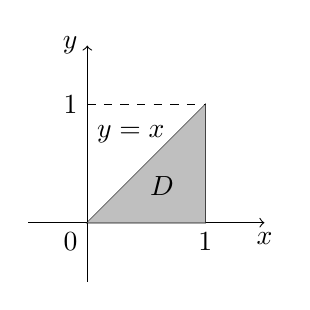
\begin{tikzpicture}[scale = 1.5]
            \draw [->] (0, -0.5) -- (0, 1.5);
            \draw [->] (-0.5, 0) -- (1.5, 0);
            \draw (0, 0) -- (1, 0) -- (1, 1) -- cycle;
            \draw [dashed] (0, 1) -- (1, 1);
            \fill [lightgray] (0, 0) -- (1, 0) -- (1, 1);
            \node [below] at (1.5, 0) {$x$};
            \node [left] at (0, 1.5) {$y$};
            \node [above right] at (0.45, 0.15) {$D$};
            \node [right] at (0, 0.75) {$y = x$};
            \node [below] at (1, 0) {$1$};
            \node [left] at (0, 1) {$1$};
            \node [below left] at (0, 0) {$0$};  
        \end{tikzpicture}
    \end{tabular}

    $f_{\xi_1}(x) = \begin{cases}
        \int\limits_0^x 2 dy = 2x, & x \in \left[ 0; 1\right] \\
        0, & x \notin \left[ 0; 1\right]
    \end{cases}$, 
    $f_{\xi_2}(y) = \begin{cases}
        \int\limits_1^y 2 dy = 2(1-y), & y \in \left[ 0; 1\right] \\
        0, & y \notin \left[ 0; 1\right]
    \end{cases}$.

    Запишемо умовні щільності: 

    $f_{\xi_1}(x/y) = \frac{f_{\vec{\xi}}(x, y)}{f_{\xi_2}(y)} = \begin{cases}
        \frac{1}{1-y}, & x \in \left[ y; 1\right], \\
        & y \in \left[ 0; 1\right)\\
        0, & \text{інакше}
    \end{cases}$,
    $f_{\xi_2}(y/x) = \frac{f_{\vec{\xi}}(x, y)}{f_{\xi_1}(x)} = \begin{cases}
        \frac{1}{x}, & y \in \left[ 0; x\right], \\
        & x \in \left( 0; 1\right] \\
        0, & \text{інакше}
    \end{cases}$.

    Умовні розподіли обох координат є рівномірними з параметрами $\left< y, 1\right>$ та $\left<0, x\right>$ відповідно.

    $E\xi_1 = \int\limits_0^1 2x^2 dx = \frac{2}{3}$,
    $E\xi_2 = \int\limits_0^1 2y(1-y) dy = \frac{1}{3}$.
    Знайдемо умовні математичні сподівання.

    $E(\xi_1 / \xi_2 = y) = \int\limits_{-\infty}^{+\infty} x f_{\xi_1}(x/y)dx =
    \frac{1}{1-y} \int\limits_y^1 x dx = \frac{1}{1-y} \cdot \frac{1-y^2}{2} = \frac{1+y}{2}$, $y \in \left[ 0; 1\right)$.

    $E(\xi_2 / \xi_1 = x) = \int\limits_{-\infty}^{+\infty} y f_{\xi_2}(y/x)dy = 
    \frac{1}{x} \int\limits_0^x y dy = \frac{1}{x} \cdot \frac{x^2}{2} = \frac{x}{2}$, $x \in \left( 0; 1\right]$.
\end{example}
\subsection{Формули повного математичного сподівання та дисперсії}
\noindent\textbf{Формула повного математичного сподівання.}
    $E(E(\xi_1 / \xi_2)) = E\xi_1$, $E(E(\xi_2 / \xi_1)) = E\xi_2$.
\begin{proof}
    Дискретний випадок:

    $E(E(\xi_1 / \xi_2)) = \sum\limits_{j = 1}^m 
    \left(
        \sum\limits_{i=1}^n x_i P\{\xi_1 = x_i / \xi_2 = y_j\}
    \right) P\{\xi_2 = y_j\} = 
    \sum\limits_{i=1}^n x_i P\{\xi_1 = x_i\} = E\xi_1$.

    Неперервний випадок:

    $E(E(\xi_1 / \xi_2)) = \int\limits_{-\infty}^{+\infty} 
    \left(
        \int\limits_{-\infty}^{+\infty} x f_{\xi_1}(x / y) dx
    \right) f_{\xi_2}(y) dy
    = \int\limits_{-\infty}^{+\infty} x f_{\xi_1}(x) dx = E\xi_1$.

    Для $\xi_2$ --- аналогічно.
\end{proof}

%\begin{remark}
%    В англомовній літературі також використовується назва «Adam's law».
%\end{remark}
\begin{example}
    Продовження попередніх прикладів.
    \begin{enumerate}
        \item Дискретний випадок:
        
        $E\xi_1 = -0.3 + 0.2 = -0.1$, $E(E(\xi_1 / \xi_2)) = -\frac{1}{6}
        \cdot0.6 = -0.1$.
    
        $E\xi_2 = 0.6$, $E(E(\xi_2 / \xi_1)) = 0.3\cdot\frac{2}{3} + 
        \frac{1}{2}\cdot\frac{3}{5} + \frac{1}{2} \cdot\frac{2}{10} = 
        0.6$.
        \item Неперервний випадок:

        $E(E(\xi_1 / \xi_2)) = \int\limits_0^1 \frac{1+y}{2} \cdot 2(1-y) dy = \int\limits_0^1 (1-y^2) dy = \frac{2}{3} = E\xi_1$,
        $E(E(\xi_2 / \xi_1)) = \int\limits_0^1 \frac{x}{2} \cdot 2x dx = \int\limits_0^1 x^2 dx = \frac{1}{3} = E\xi_2$.
    \end{enumerate}
\end{example}


Крім умовного математичного сподівання розглядають
\emph{умовні дисперсії} --- міра розсіювання однієї випадкової величини 
за умови того, що інша набула певне значення.

\noindent\textbf{Формула повної дисперсії.}
    Нехай $\xi_1$, $\xi_2$ --- випадкові величини та $D\xi_1 < +\infty$. 
    Тоді
    $D\xi_1 = E(D(\xi_1/\xi_2)) + D(E(\xi_1 / \xi_2))$.

\begin{proof}
    $D\xi_1 = E\xi_1^2 - (E \xi_1)^2 = 
    E(E(\xi_1^2 / \xi_2)) - (E(E(\xi_1/\xi_2)))^2 = 
    E(D(\xi_1/\xi_2) + (E(\xi_1/\xi_2))^2) - (E(E(\xi_1/\xi_2)))^2 = 
    E(D(\xi_1 / \xi_2)) + (E(E(\xi_1/\xi_2)^2) - 
    (E(E(\xi_1 / \xi_2)))^2) = E(D(\xi_1/\xi_2)) + D(E(\xi_1/\xi_2))$.
\end{proof}


%\begin{remark}
%    В англомовній літературі також використовується назва Eve's law».
%\end{remark}

\subsection{Незалежність координат випадкового вектора}

Розглядаємо випадок $n=2$, $\vec{\xi} = \left(\xi_1, \xi_2\right)^T$.

Необхідною і достатньою умовою незалежності координат, як вже було розглянуто, є 
$F_{\vec{\xi}}(x, y) = F_{\xi_1}(x)\cdot F_{\xi_2}(y)$.

З цього випливає, що в разі незалежності координат $F_{\xi_1}(x/y) = F_{\xi_1}(x)$, 
$F_{\xi_2}(y/x) = F_{\xi_2}(y)$.

\noindent\textbf{Дискретний випадок: }

$P\{\xi_1 = x_i, \xi_2 = y_j\} = P\{\xi_1 = x_i\}\cdot P\{\xi_2 = y_j\}$ 
$\forall i,j$.
З цього випливає, що:

\begin{enumerate}
    \item $P\{\xi_1 = x_i / \xi_2 = y_j\} = 
    P\{\xi_1 = x_i\}\cdot P\{\xi_2 = y_j\}$.
    \item $E(\xi_1 / \xi_2 = y_j) = E\xi_1$,
    $E(\xi_2 / \xi_1 = x_i) = E\xi_2$.
\end{enumerate}

\noindent\textbf{Неперервний випадок: }

$f_{\vec{\xi}}(x, y) = f_{\xi_1}(x)\cdot f_{\xi_2}(y)$.
З цього випливає, що:

\begin{enumerate}
    \item $f_{\xi_1}(x/y) = f_{\xi_1}(x)$,    
    $f_{\xi_2}(y/x) = f_{\xi_2}(y)$.
    \item $E(\xi_1 / \xi_2 = y) = E\xi_1$, 
    $E(\xi_2 / \xi_1 = x) = E\xi_2$.
\end{enumerate}

\noindent Для $n$-вимірного випадку ($n > 2$):
$\forall i,j$: $F_{\xi_i\xi_j}(x_i, x_j) = F_{\xi_i}(x_i)\cdot F_{\xi_j}(x_j)$ --- 
попарна незалежність.

\begin{definition}
    Координати $\xi_1, \xi_2, ..., \xi_n$ є \emph{незалежними у сукупності} 
    тоді і тільки тоді коли $F_{\vec{\xi}}(\vec{x}) = 
    \prod\limits_{k=1}^n F_{\xi_k}(x_k)$.
\end{definition}
У випадку незалежності у сукупності координат неперервного випадкового вектора має місце аналогічна
властивість для щільності:
\begin{equation*}
    f_{\vec{\xi}}(\vec{x}) = \frac{\partial^nF_{\vec{\xi}}(\vec{x})}
    {\partial x_1...\partial x_n} \Rightarrow 
    f_{\vec{\xi}}(\vec{x}) = \prod\limits_{k=1}^n f_{\xi_k}(x_k)
\end{equation*}

\noindent\textbf{Твердження.}
    З незалежності у сукупності випливає попарна незалежність
    (зворотнє твердження, взагалі кажучи, не має місця).
\begin{proof}
    $F_{\xi_i\xi_j}(x_i, x_j) = F_{\vec{\xi}}(+\infty, ..., +\infty, x_i, 
    +\infty, ..., +\infty, x_j, +\infty, ..., +\infty) = $

    $= F_{\xi_1}(+\infty)...F_{\xi_{i-1}}(+\infty)F_{\xi_i}(x_i)
    F_{\xi_{i+1}}(+\infty)...F_{\xi_{j-1}}(+\infty)F_{\xi_{j}}(x_j)
    F_{\xi_{j+1}}(+\infty)F_{\xi_n}(+\infty) = $
    
    $= F_{\xi_i}(x_i)\cdot F_{\xi_j}(x_j)$.
\end{proof}

\begin{remark}
    З незалежності у сукупності випливає некорельованість.
\end{remark}